\chapter{Ancora sull'AI}

\section{AI or not AI This is the Dilemma}

\subsection{Il Watermark}

\dfn{Watermark}{
  Il watermark consiste in cambiamenti non visibili in alcuni pixel chiavi che possono essere individuati dalla macchina.
}

\begin{figure}[H]
    \centering
    
\includegraphics[scale=0.5]{02E/wm.png}
    \caption{Immagine con watermark.}
\end{figure}

\nt{Uno dei provvedimenti dell'amministrazione Biden per "difendersi" da watermark è stato quello di dire: inseriamo del watermark che indichi se un'immagine è AI-generated.}

\qs{}{Questa è una soluzione ragionevole?}

\begin{itemize}
  \item Se è possibile introdurlo allora esisterà un AI in grado di rimuoverlo. 
  \item Questa proposta garantisce Microsoft, openAI, Google che se ne lavano le mani. Però le aziende non americane non hanno alcun obbligo di applicare il watermark.
  \item Inoltre il fatto che una foto abbia il watermark, in un'epoca di cospirazionismo, non significa nulla\footnote{God, how much I hate humanity.}.
\end{itemize}

\subsection{Il Copyright}

Tutti i vari modelli di AI generativa sono stati addestrati su tutti i dati del mondo, principalmente il web (anche su materiale soggetto a copyright). Per esempio alcuni siti come z-library o il web archive\footnote{Entrambi consigliatissimi, da visitare almeno una volta nella vita, sono la nuova biblioteca di Alessandria.} in cui sono presenti contenuti piratati. I vari LLM hanno probabilmente assorbito anche quei contenuti. Ovviamente quella merda che è Google ha detto: eh, ma se è lì sul web allora lo posso prendere, se non lo volevano non lo dovevano pubblicare (a parte che è l'esatto opposto del meccanismo di copyright, ma forse non si rendono conto che è la stessa argomentazione che utilizzano gli stupratori nei confronti della loro vittima). Oppure openAI che chiede alle persone di indicare quali pagine non vogliono sia preso dal crawler. Tuttavia questo non funziona, per esempio con i siti di mirroring.

\begin{figure}[H]
    \centering
    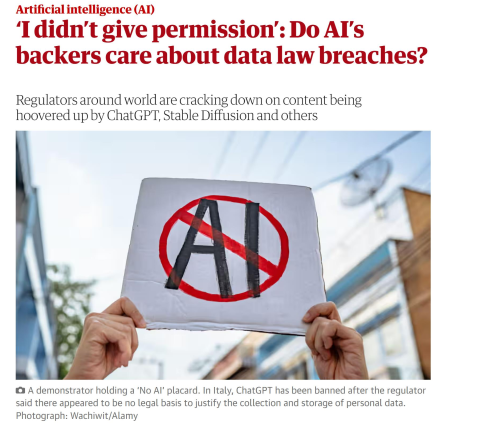
\includegraphics[scale=0.65]{02E/ai.png}
    \caption{Protestante con cartello.}
\end{figure}

\section{Breve Prospettiva Storica}

\paragraph{Nell'antichità:}

\begin{itemize}
  \item In Mesopotamia l'homo sapiens ha iniziato la sua età d'oro. 
  \item Circa 5000 anni fa nasce la scrittura. 
  \item Un'altra capacità che gli esseri umani sviluppano è quella di creare finzioni (storie, miti, patrie, religioni) allo scopo di aumentare la coesione tra di loro. I templi mesopotamici non erano così diversi dalle corporations moderne: avevano possedimenti, si occupavano di dare lavoro, etc. 
  \item Schiavitù nell'epoca romana: erano un oggetto, una proprietà. Se un nobile veniva ucciso da uno schiavo allora tutti gli altri schiavi dovevano venire giustiziati. 
  \item Commons: le parti di terra, mare, etc. non sono di una persona, ma della comunità.
  \item Facendo un salto avanti, nel 1968, Garret Hardin pubblica un libro in cui sostiene che i commons non  possono funzionare perché le risorse sono limitate (giustifica la proprietà privata). Una ventina di anni dopo Elinor Ostrom rispose che i sistemi di commons si autoregolano e quindi nessuno può approfittarne.
\end{itemize}

\paragraph{Dal feudalesimo:}

\begin{itemize}
  \item Gutenberg nel 1455 inventa la stampa a caratteri mobili. Viene usata per stampare la Bibbia, il ché porta alla diffusione della religione a prescindere dalla chiesa e poco dopo alla rivoluzione protestante di Lutero.
  \item I commons vengono dati a signori feudali sviluppando il latifondismo e aumentando la povertà degli abitanti dei villaggi. 
  \item Questo si ricollega a temi come l'espropriazione dei beni comuni (e.g. l'IA che fa concorrenza alle persone e viola il copyright).
  \item Non esistendo lo stato di diritto ogni feudatario si fa le sue regole.
  \item Nel '500 inizia la conquista delle Americhe. Si deve leggere un editto prima di assaltare i villaggi (questo è ripreso da aziende moderne come Google).
  \item A inizio del '600 Cartesio definisce il piano cartesiano (rendendo la geometria una questione di matematica). Oltre a questo sdogana il tabù relativo allo studio dei cadaveri. Il corpo, da entità sacra, diventa un qualcosa di studiabile. Introduce anche la visione del mondo come un grande orologio. Ma sostiene che linguaggio e ragionamento, in quanto dominio della mente e non del corpo, non sono studiabili.
  \item Successivamente, Julien Offray de La Mettrie, pubblica un trattato in cui parla di come la mente possa essere vista come una macchina modellabile. 
  \item Newton sfrutta l'idea di Cartesio e riconduce corpi celesti all'esperienza comune. Rendendo umano il divino. 
\end{itemize}

\paragraph{La rivoluzione industriale:}

\begin{itemize}
  \item Adam Smith propose due teorie:
    \begin{itemize}
      \item Teoria della separazione dei lavori: persone specializzate fanno sempre la stessa cose. 
      \item La mano invisibile del mercato: elogio dell'imprenditoria.\footnote{Non è in grado di spiegarlo meglio perché è una stronzata.}
    \end{itemize}
  \item Tra la fine del '700 e l'inizio dell'800 nasce il \fancyglitter{luddismo}: un movimento di protesta operaia. 
  \item Il telaio ampio veniva utilizzato per il lavoro minorile, c'erano guerre in tutta europa, etc.
  \item Nel 1791 viene adottato il primo emendamento  che preveniva una serie di leggi. Il \fancyglitter{Panopticon} serve per sorvegliare potenzialmente tutti.
  \item 1833: New York Sun redatto da Benjamin Day. Costava meno, ma aveva la pubblicità all'interno. Era pieno di notizie scandalistiche, cronache giudiziarie, etc.
  \item 1860: Jules Cheret viene pagato per pubblicare manifesti pubblicitari. Dopo anni la popolazione di parigi si lamenta che questi manifesti rovinavano il panorama.
  \item 1890: viene pubblicizzata la Patent Medicine, generalmente truffe, verrà regolamentata nel 1906 con il Food and Drugs Act.
  \item 1893: Emile Durkheim mostra come la divisione dei lavori si sia spostata dalle fabbriche alla società. Si sono create dipendenze e coesioni tra le persone. Questo è un rischio perché nel momento in cui il padrone sostituirà i dipendenti con i robot questa mutua dipendenza si romperà.
  \item A fine '800 nasce il telefono come broadcast. Battaglia sui brevetti vinta da Bell. 
  \item Il telefono rimpiazza il telegrafo e crea un nuovo monopolio. 
  \item Nascita dei vari monopoli: treni, petrolio (Rockfeller), etc. 
  \item Herbert Spencer giustifica i monopoli con il \fancyglitter{darwinismo sociale}: il mercato ha le sue leggi per cui esistono vincitori e sconfitti. Punta a limitare la democrazia e sfocia nell'eugenetica.
  \item Sherman Act: tenta di limitare i monopoli. Nel 1911: azione antitrust che dissolve la standard oil. 
  \item Qualche anno dopo la Federal Trade Commission per regolare la concorrenza. 
  \item Theodore Vail: per le telecomunicazioni è utile avere un player che offra garanzie al pubblico. 
\end{itemize}

\paragraph{Le automobili:}

\begin{itemize}
  \item Inizialmente come bene di lusso. 
  \item Le strade però erano un bene comune, le auto erano pericolose. 
  \item Vengono obbligati i possessori di automobili a farle precedere da una persona con una bandiera rossa per segnalarne l'arrivo. 
  \item Viene fatta una grande campagna in cui venivano criticate le persone che vivevano per la strada. Viene creato il reato di camminamento in mezzo alla strada.
  \item Ford crea la produzione di massa delle automobili.
  \item Ai giorni nostri ci sono stati movimenti riguardo le piste ciclabili per reclamare la strada.
\end{itemize}

\begin{figure}[H]
    \centering
    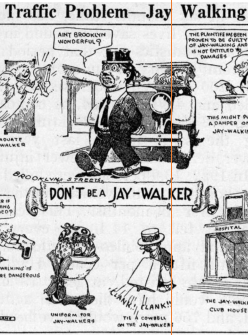
\includegraphics[scale=0.7]{02E/traffic.png}
    \caption{Reato di Jay-Walking.}
\end{figure}

\paragraph{La modernità:}

\begin{itemize}
  \item 1908: Edison Motion Picture Patents, nasce il cinema. 
  \item Veniva bloccato l'import delle pellicole, il cinema era un monopolio. 
  \item 1912: Zukor crea la Paramount, dando vita al cinema statunitense. Si passa a un altro monopolio\footnote{Nothing ever happens, uh?}.
  \item Zio Sam: chiamata alle armi. La pubblicità viene usata a scopi propagandistici.
  \item Volontà di guerra, bisogna allinearsi alla volontà dello stato. 
  \item Contro la pubblicità si schiera Walter Lippmann mostrando come essa sia uno strumento di propaganda. 
  \item 1935: Riefenshal's Nazi Propaganda film. 
  \item La radio fu molto usata da Goebbels,  ministro della propaganda nella germania nazista.
\end{itemize}















